\documentclass{article}

\usepackage{graphicx}
\usepackage{hyperref}
\usepackage{titling}

\newcommand{\name}{Virtuous Hummingbird}

\setlength{\droptitle}{-30mm}
\title{Product Requirements \\ \textit{for} \\ \name{}}
\author{\href{https://github.com/wintertideheir}{wintertideheir}}

\begin{document}

\maketitle

\name{} is a program for the organization and advancement of personal virtue.
By virtue, we mean the virtues of virtue ethics, personal qualities indicating a pattern of repeated behavior.
These qualities are related causally to form a hierarchical tree of virtues. 
The simple nature of virtues and virtue trees makes virtue ethics an unusually intuitive and practical ethical theory.
By presenting a way to create, edit, visualize, and track these virtues, \name{} facilitates living a virtuous life.

\tableofcontents

\section{Background}

\name{} was concieved as an improvement on another concept-mapping system, Cmap, for mapping virtue ethics.

Cmap is a trademark applied to a series of products created by the Florida Institute for Human and Machine Cognition.
Cmap products are intended to empower users to represent knowledge as concept maps.
CmapTools, a Cmap product, is a desktop application that allows users to view and manipulate concept maps.
Because Cmap products could represent any knowledge, CMapTools was adopted as a tool to research virtue ethics.

However, Cmap products are only optimized for general use.
When faced with high volume graphs in virtue ethics, the representations they unnavigatable and unusable.
CmapTools is also limited in it's ability to parse concept maps and generate new insights.
In the long term, CmapTools is not a programs that can be easily extended to perform other functions.

A new kind of concept-mapping software was concieved, optimized for virtue ethics and extensible with utilities.
To avoid information overload, the concept map would be represented as simple nodes.
The information associated with these nodes would be specific to the class of the node.

\section{Purpose}

\name{} targets the problem of mapping virtue ethics.
Mapping is the process of creating symbolic representations of objects and their relationships.
Mapping virtue ethics is the process of creating symbolic representations of virtues, vices, goods, and their relationships.
Common mapping systems and software are ineffective at mapping virtue ethics because one's understanding of a large number of objects can shift rapidly.
For example, we could map the physical virtues by describing how they relate to different anatomical structures.
We could then use that mapping to decide which skills we're deficient in and therefore what exercises we ought to do.
Then, perhaps, after a sojourn in the land of exercise science, we decide that we would be better representing physical virtues by what kinetic chain or motion they rely on.
How would we transform our existing map, and how would we preserve the utilities we'd already derived from it?
The problem of mapping virtue ethics is the problem of creating and preserving utility across significant changes to the representation.

\name{} improves on existing concept-mapping software by restricting what kinds of maps can be created.

First, all concept-maps are directed graphs, and the primary map is acyclic.
Directed graphs have an inherent structure that facilitates writing predictable sequence-based utilities.
Acyclic graphs furthermore prevent utilities from having to arbitrarily break endless loops.
These requirements make \name{} predictable and therefore easy to use.

Second, only certain classes of objects and relationships can be represented.
Because \name{} is primarily concerned with virtue ethics, representable objects include virtues, vices, goods, activities, and metrics.
Each representable object has a fixed internal structure made of simple fields to ensure consistent behavior for utilities.
The map also has an macroscopic structure, enforced by the small number of representable relationships.
The center of the primary map is a tree of virtues and vices, of which each can have an associated tree of goods, activities, or metrics attached.

By standardizing on what kinds of maps \name{} will accept, we have streamlined the process of creating representations of virtue.
To create a virtue map, users will first create a tree of virtues and a tree of goods.
Then they will create activities and metrics for any virtue or good.
Editing, navigating, and viewing the map involve selecting an object type and specifying additional parameters based on the object.

\section{Objectives}

\begin{itemize}
    \item Demonstrate a real world example of a virtue graph with at least 1,000 virtues.
    \item Represent the virtues presented by Aristotle in \textit{Nicomachean Ethics}.
\end{itemize}

\section{Features}

\begin{figure}[h]
    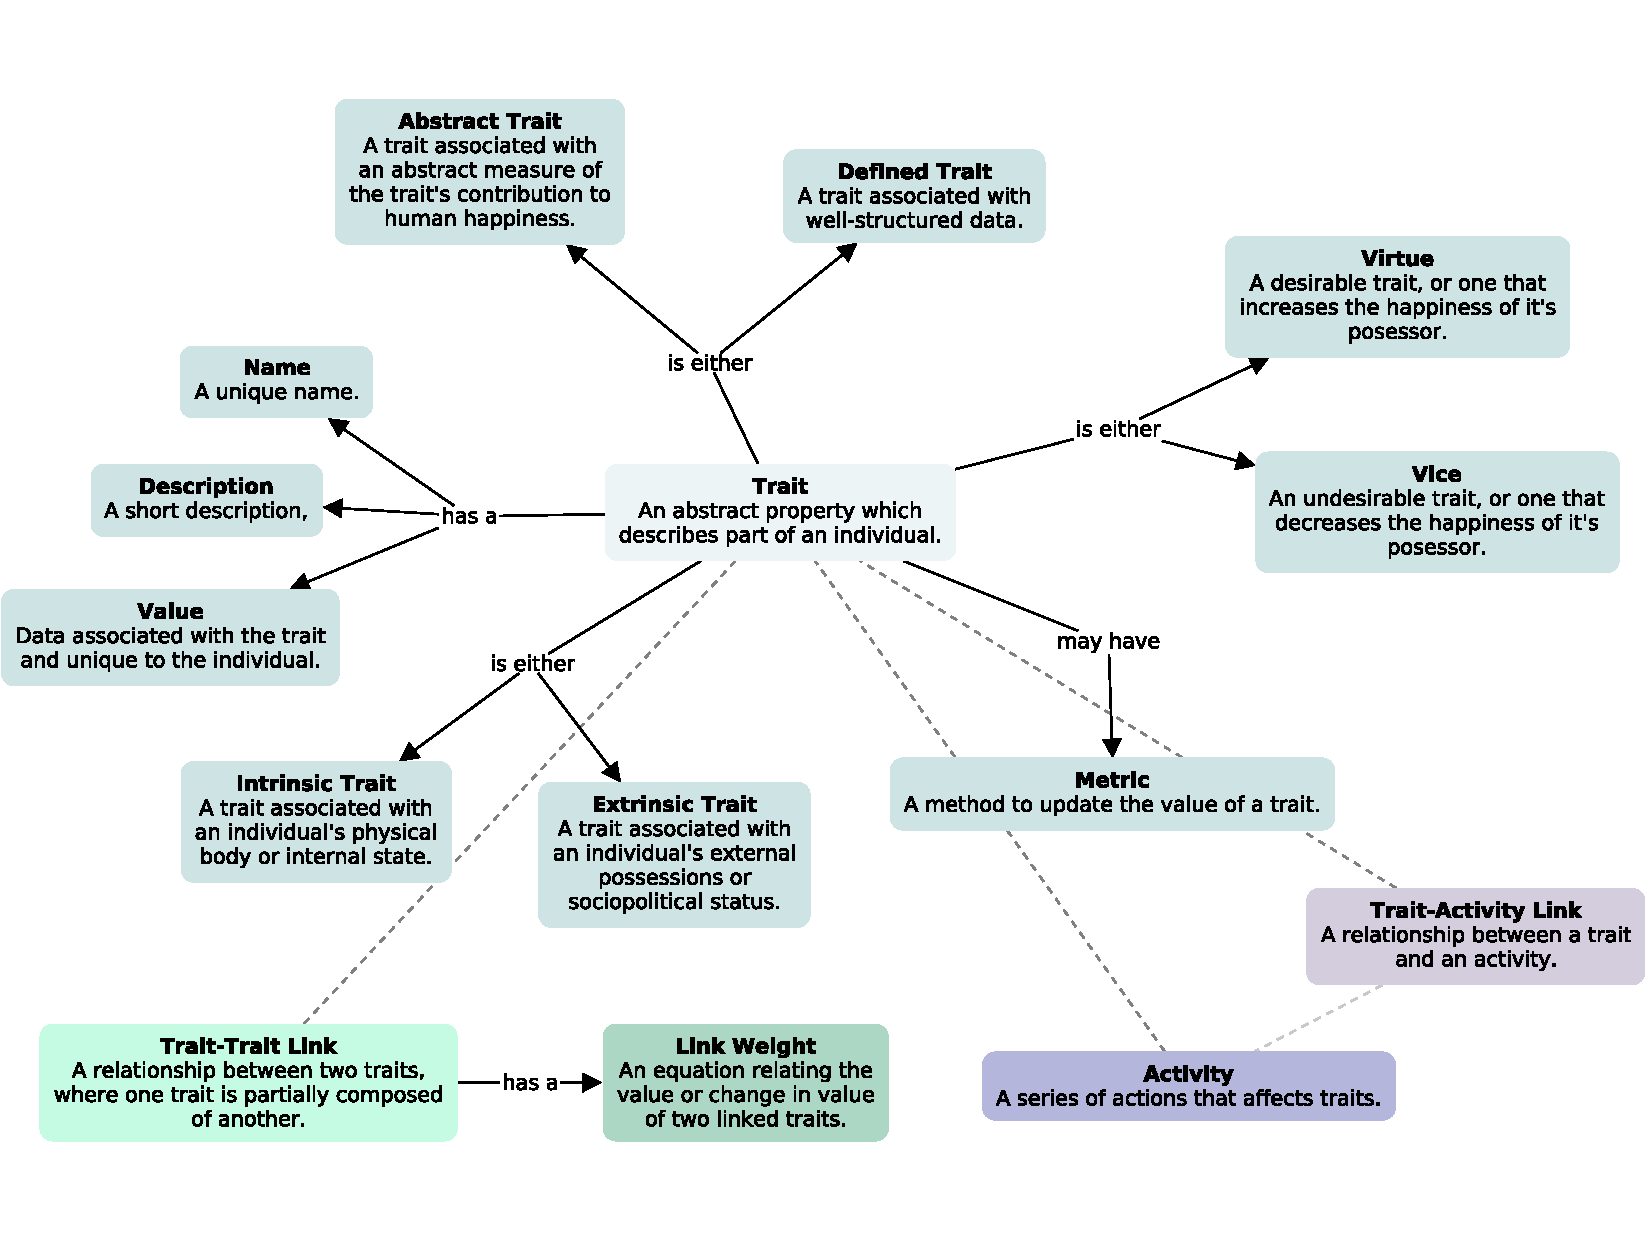
\includegraphics[width=\linewidth]{classes.pdf}
    \caption{Classes}
    \label{fig:classes}
\end{figure}

\section{Comparables}

% What other products offer similar features?

\section{Summary}

% Summarize who has what problem, and how the product solves it.

\end{document}
